\documentclass[a4paper, 12pt, twoside]{report}

\usepackage[top=2.5cm, bottom=3cm, left=3cm, right=2cm]{geometry}
\usepackage{mathtools}
\usepackage{amsthm}
\usepackage[bitstream-charter]{mathdesign}
\usepackage[pdftex]{graphicx}
\usepackage{fixltx2e}
\usepackage{afterpage}
\usepackage[acronym,nomain]{glossaries}
\usepackage{latexsym}
\usepackage{times}
\usepackage{amsmath}
\usepackage{subfigure}
\usepackage{multirow}
\usepackage{rotating}
\usepackage[table]{xcolor}
\usepackage[acronym,nomain]{glossaries}
\usepackage{setspace}
\usepackage[nottoc]{tocbibind}
\usepackage[toc, page]{appendix}
\usepackage{setspace}
\usepackage{xcolor}
\usepackage{natbib}

\usepackage{color}
\usepackage{hyperref}
\hypersetup{
	colorlinks=true,	% make the links colored
	linkcolor=blue,		% color TOC links in blue
	urlcolor=red,		% color URLs in red
	linktoc=all		% 'all' will create links for everything in the TOC
}

\newcommand{\q}[1]{``#1''}
\newcommand{\HRule}{\rule{\linewidth}{0.5mm}}
\newcommand{\scDiaeresis}[1]{\"{#1}}

\newenvironment{dedication}
{
	\clearpage		% we want a new page
	\thispagestyle{empty}	% no header and footer
	\vspace*{\stretch{1}}	% some space at the top
	\itshape		% the text is in italics
	\centering		% flush to the right margin
}
{
	\par			% end the paragraph
	\vspace{\stretch{3}}	% space at bottom is three times that at the top
	\clearpage		% finish off the page
}
\newtheorem{theorem}{Theorem}
\newtheorem{remark}{Remark}
\newtheorem{definition}{Definition}
\newtheorem{corollary}{Corollary}
\newtheorem{lemma}{Lemma}
\newtheorem{note}{Note}
\makeglossaries

\setcounter{tocdepth}{3}
\setcounter{secnumdepth}{3}

\begin{document}

\begin{titlepage}

\begin{center}
\HRule \\[0.4cm]
{\huge \bfseries \textbf{Image Integrity Analysis with BlockChain Technology}  \\[0.4cm] }
\HRule \\[1cm]
\end{center}

\vspace{0.2cm}

\begin{center}
{\large{Bachelor Thesis}}
\end{center}

\vspace{0.25cm}

\begin{center}
\large{\textit{Submitted By}}
\end{center}

\vspace{0.35cm}

\begin{center}
{\large{Anuj Kr. Pathak\\\&\\Sayan Shankhari}}
\end{center}

\vspace{0.25cm}

\begin{figure}[h]
\centering

\includegraphics[width=0.25\textwidth]{./img_src/iiitk.png}
\end{figure}

\vspace{0.5cm}

\begin{center}
{\textit{\Large{A thesis submitted to}}} \\
\end{center}

\vspace{0.25cm}

\begin{center}
\Large{Indian Institute of Information Technology Kalyani} \\
\end{center}

\vspace{0.35cm}

\begin{center}
\textit{\large {for the partial fulfillment of the degree of}} \\
\vspace{0.8cm}
\textbf{\Large{Bachelor of Engineering in Computer Science}} \\
\end{center}

\begin{center}
\textbf{{\large{in}}}
\end{center}

%\vspace{0.1cm}
\begin{center}
\textbf{\Large{Department of Computer Science and Information Technology}} \\
\end{center}

\vspace{0.5cm}

\begin{center}
\Large{May, 2019}
\end{center}

\end{titlepage}

\newpage
\begin{dedication}
\textit{To my beloved parents and friends who have supported me and prayed for my success\\ throughout my life.}
\end{dedication}

\newpage
\chapter*{}
%\setcounter{page}{1}
\pagenumbering{roman}
\begin{center}
\textbf{\textsc{\Large Certificate}}\\[0.75cm]
\end{center}

\onehalfspacing This is to certify that the thesis entitled
\textbf{\q{Image Integrity Analysis with BlockChain Technology}} being submitted by undergraduate students \textbf{Anuj Kr. Pathak} (Reg. No.: 000000102) and \textbf{Sayan Shankhari} (Reg. No.: 00000121) in the Department of Computer Science and Information Technology, Indian Institute of Information Technology Kalyani, Nodia, 741235, India, for the award of \textbf{Bachelors of Technology} in \textbf{Computer Science \& Engineering}, is an original research work carried by them under my supervision and guidance. The synopsis has fulfilled all the requirements as par the regulation of \textbf{IIIT Kalyani} and in my opinion, has reached the standards needed for submission. The works, techniques and the results presented have not been submitted to any other university or Institute for the award of any other degree or diploma.\\
\bigskip
\bigskip
\bigskip
\bigskip
\bigskip
\bigskip
\bigskip
\begin{flushleft}
\bigskip
-------------------------------\\
(\textbf{Dr. Imon Mukherjee})\\
\smallskip
Assistant Professor\\
Department of Computer Science and Information Systems\\
Indian Institute of Information Technology Kalyani\\
IIIT Kalyani Campus, West Bengal 741235, India.
May 2019\\
\end{flushleft}

\newpage
\chapter*{}
%\setcounter{page}{1}
%\pagenumbering{roman}
\begin{center}
\textbf{\textsc{\Large Declaration}}\\[0.75cm]
\end{center}

\onehalfspacing
We hereby declare that the work being presented in this thesis entitled, \textbf{\q{Image Integrity Analysis with BlockChain Technology}}, submitted to Indian Institute of Information Technology Kalyani in partial fulfilment for the award of the degree of Bachelor of Technology in Computer Science and Engineering during the period from July, 2018 to May, 2019 under the supervision of Dr. Imon Mukherjee, Department of Computer Science and Engineering, Indian Institute of Information Technology Kalyani, West Bengal 741235, India, does not contain any classified information.

\bigskip
\bigskip
\bigskip
\bigskip

\noindent
-------------------------------- \hfill -------------------------------- \\
\textbf{Anuj Kumar Pathak} \hfill \textbf{Sayan Shankhari} \\
39/CSE-15145 :: 00000102 \hfill 67/IT-15026 :: 00000121 \\
Computer Science and Engineering, \hfill Information Technology, \\
Indian Institute of Information \hfill Indian Institute of Information\\
Technology Kalyani, \hfill Technology Kalyani, \\
WEBEL IT Park, West Bengal \hfill WEBEL IT Park, West Bengal \\
741235 India \hfill 741235 India

\bigskip
\bigskip
\bigskip
This is to certify that the above statement made by the candidate is correct to the best of my knowledge.

\bigskip
\begin{flushleft}
\bigskip
\bigskip
------------------------------- \\
(\textbf{Dr. Imon Mukherjee}) \\
\smallskip
Assistant Professor \\
Department of Computer Science and Information Systems \\
Indian Institute of Information Technology Kalyani \\
IIIT Kalyani Campus, West Bengal 741235, India \\
May 2019 \\
\end{flushleft}

\chapter*{Acknowledgments}
First of all, We would like to take this opportunity to thank my supervisor Dr. Imon Mukherjee without whose effort this thesis would not have been possible. We are so grateful to him for working tirelessly after us, clearing our doubts whenever and wherever possible. We are most grateful to Department of Computer Science and Information Technology, Indian Institute of Information Technology Kalyani, West Bengal, 741235, India, for providing us this wonderful opportunity to complete our bachelor thesis. We would like to thank our friends for providing us help as and when required. We would like to thank our team mates for being a great motivators and great friends. \\
\\
\linebreak And last but the biggest of all, We want to thank our parents, for always believing in us and letting us do what we wanted, but keeping a continuous check that we never wandered off the track from my goal. \\

\bigskip
\bigskip
\bigskip
\bigskip

\noindent
-------------------------------- \hfill -------------------------------- \\
\textbf{Anuj Kumar Pathak} \hfill \textbf{Sayan Shankhari} \\
39/CSE-15145 :: 00000102 \hfill 67/IT-15026 :: 00000121 \\
Computer Science and Engineering, \hfill Information Technology, \\
Indian Institute of Information \hfill Indian Institute of Information\\
Technology Kalyani, \hfill Technology Kalyani, \\
WEBEL IT Park, West Bengal \hfill Webel IT Park, West Bengal \\
741235 India \hfill 741235 India


%\singlespacing
\pagebreak \tableofcontents
\pagebreak \listoffigures
\newpage
\chapter*{Abstract}
With the digitalization any historical record are available in the form of collection of bits. Any document can be stored in advanced electronic devices like computers, smart phones file systems as files. The most used or popular files are media files (image, audio, video). For the lack of true information and experience or bad ethics of mind the number of digital scams is getting higher in developing country like India. So the data files need to be protected somehow somewhere and also there should be a system that will veryfy the requested file. So we started with the simplest media format \textit{i.e.} Image. Making a centrral database can be unreliable because the system can be breached and the data might be changed no matter how advanced and protective the protocols are. So we took the concept from advanced decentralized architecture of BlockChain mostly BitCoin.
A purely peer-to-peer version of online data would allow online transactions to be sent directly from one node to another without going through a central authority. Digital signatures provide part of the solution.
The network timestamps transactions by hashing them into an ongoing chain of hash-based proof-of-work, forming a record that cannot be changed without redoing the proof-of-work. The longest chain not only serves as proof of the sequence of events witnessed, but proof that it came from the largest pool of CPU power. As long as a majority of CPU power is controlled by nodes that are not cooperating to attack the network, they'll generate the longest chain and outpace attackers. The network itself requires minimal structure. Messages are broadcast on a best effort basis, and nodes can leave and rejoin the network at will, accepting the longest proof-of-work chain as proof of what happened while they were gone.
To prevent the action against one of the biggest issues in India of Fake Media (Image, Sound) Scam. This project tries to find a way to prevent it with a new upcoming technology starting with image files.

\textbf{Keywords:} Peer-to-Peer network, Proof-of-work, Proof-of-Stake, Distributed Ledger, Concensus Mechanism, Hash Function, Video Formatting, Image File formats, Watermarking, WebServer.

% \afterpage{\null\newpage}

\chapter{Introduction}
\label{Ch1}
%\setcounter{page}{1}
\pagenumbering{arabic}

\bigskip
\bigskip
\bigskip

This chapter presents the introduction of the thesis that includes the brief description of BlockChain, and the adopted approach to address the problems. This chapter also presents the scope of this thesis and the contributions of the thesis.

Image integrity is the task of checking if the image file's bits are changed or not at any point. A digital file might change by platforms. This would be fully online system. Nowadays with increasing people in digital world the editing softwares are getting smart. Most of the files that might be non-editable in some operating systems or file systems, but the so called hackers or masters of electronic devices have file systems that can easily access and change any file data. So in that way the media files can not be checked for integrity. And also while the images are shared in different platforms, the files' data might be changed according to their protocols for data compression or security.

The proposed system in this thesis will help us to detect those shared files and compare them not bit by bit, but context wise and signature wise. That means if one shares an image both our system as well as one of those online platforms and download them as separate file and check in our system, it should return truth values if data portion are same or atleast 95\% same. The system we are introducing the social media like platform that have the capability to store images and show them in news feed. There is a option for every photo to download in user's computer or mobile devices and after sharing and getting back the person can check if the file is intact or not in our proposed system by the digital signature.

\section{Scope of Discussion}
This thesis focuses on building a hybrid architechture inspired by one of the major implementations of BlockChain i.e. BitCoin~\cite{nakamoto2008bitcoin}. By the advancement of PHP (Hypertext PreProcessor) and JS (JavaScript) which are the basic building languages or platforms that can be run in any modern devices, it might be quite easy to make a peer-to-peer web-api (Application Programming Interface) running like bitcoin decentraized network as well as social media platform that might be a real Truth Machine. While comparing image files data we will first compress the data using our own protocol and compare by bit matching Euclid, or Deep CNN (Convolutional Neural Network).

\section{Methodological Approach}
The system that we are trying to build is capable of processing, storing and showing image files. Not only that, it also allows viewers to veryfy his own copy of the image. It is not easy to store and veryfy in a moment and it is about impossible to change the whole blockchain, because the miners have their own copy of the public ledger and their processed computation powers in their computers. The automated server should back up its data from both the Virtual miners as well as remote miners' computers. The studied and inspired technologies are discuussed in the thesis.

\section{Thesis Contribution}
The main contributions of this thesis includes
\begin{enumerate}
\item Proposes an user anonymity-preserving algorithm to be a part of Video Integrity Program.
\item Formally analyzes the security of the newly designed protocol as well as its performance.
\item The scheme, as compared to the existing schemes, not only authenticates the users but, also establishes a session key between the user and the System after successful mutual authentication.
\item The scheme provides many security and robustness features of user authentication and Block Processing scheme for BCTs.
\item No installation required to be a part of the system, except you want to be the miner.
\end{enumerate}

\section{Roadmap of the Thesis}
The structure of the thesis is as follows:
\begin{enumerate}
\item The Chapter \ref{Ch1} is an introductory part which discusses the scope of the thesis, about the contribution of this thesis and the motivation for writing it.
\item The Chapter \ref{Ch2} provides the background of Image integrity security aspects of it and previous works.
\item The Chapter \ref{Ch3} introduces the proposed authentication framework after highlighting the motivations behind this work.
\item The implementation of Chapter \ref{Ch5}, where an informal implementation of the proposed protocol has been discussed.
\item The Chapter \ref{Ch6} comprises of the conclusion and further work of the Project in future.
\end{enumerate}

\section{BlockChain}
A BlockChain or \textbf{\q{The Truth Machine}} ~\cite{the_truth_machine} can be broadly described as a peer-to-peer network of nodes that makes a collaborative effort in sensing certain specified chain of blocks of data around its periphery and thereby controls the surrounding environment.
Accrrding to Wikipedia~\cite{blockchain_wiki} a blockchain, originally block-chain, is a growing list of records, called blocks, which are linked using cryptography. Each block contains a cryptographic hash of the previous block, a timestamp, and transaction data (generally represented as a Merkle tree).
In BlockChains, each node consists of processing capability, it may contain multiple types of memory like program, data and memories, having a Web-Service transceiver, Client-side processors, and a power source. The nodes communicate with each other using web-services and self-organized.
There are certain nodes called miners that veryfies each transactions or entry of data in the chain and are the most reliable personnel in the network who always have the updated copy of blocks of data.

\begin{figure}
\begin{center}

\includegraphics[width=0.5\textwidth]{./img_src/blockchain.jpg}
\end{center}
\caption{Overview of Block-Chain Technology (BCTs).}
\end{figure}

Some of the underlying concepts of the BlockChain especially BitCoin (the most popular implementation of BlockChain) and some other important technology are briefed.

\subsection{Peer-to-Peer Network}
This is the internet protocol that connects different logged in users as a node which is having some computation power. The users who are only uploading and verifying may have computer or smartphone, but the verifiers or the miners must have to work on computer with sufficient amount of computation power.

\subsection{Transactions}
Everything in crypto-currency comes under transactions, i.e. someone is sending some amount of money to someone else at some time. So a basic or overall transaction data can be structured as,

\fbox{\colorbox{lightgray}{\parbox[b][4cm][c]{0.50\linewidth}{
\textbf{\texttt{\noindent Transaction :: \{\\
\hspace*{1cm} \textless Transaction\_id\textgreater,\\
\hspace*{1cm} \textless TimeStamp\textgreater,\\
\hspace*{1cm} \textless Sender\_Id\textgreater,\\
\hspace*{1cm} \textless Receiver\_Id\textgreater,\\
\hspace*{1cm} \textless Amount\_Unit\textgreater\\
\noindent \}}}
}}}

This transaction details is send to every peer to verify. If they heard already about it, it is true, or it is false (same as women's un-manipulated gossip in village). If more than 50\% population declare it true, then it is allowed to be in the Public Ledger.

\subsection{Public Ledger}
This is the publicly shared record of transactions kept as a list of blocks. At a particular point of time everybody (every node), who are connected to the network, should have a same copy of ledger in their own devices of what server has. Whenever a new person logs into the network aotomatically the server forces to update the ledger to the person's device. So basically the ledger is the chain file.

\subsection{Chain of Blocks}
It means list of blocks of data having some common part with previous and next block. This is like Single-way linked-list(every node consists of data and program memory address to the next node). Every block contains a number of transactions and many more things.

\fbox{\colorbox{lightgray}{\parbox[b][6cm][c]{0.75\linewidth}{
\textbf{\texttt{\noindent Block :: \{\\
\hspace*{1cm} \textless Block\_Id\textgreater,\\
\hspace*{1cm} \textless TimeStamp\textgreater,\\
\hspace*{1cm} \textless Merkle\_Root\textgreater,\\
\hspace*{1cm} \textless Verifier\_Id\textgreater,\\
\hspace*{1cm} \textless Nonce\_Value\textgreater,\\
\hspace*{1cm} \textless Previous\_Hash\textgreater,\\
\hspace*{1cm} \textless Current\_Hash\textgreater,\\
\hspace*{1cm} \textless Data :: ANumberOfTransactions\textgreater\\
\noindent \}}}
}}}

So it is kind of backword linked-list which is propagating by having the previous block's kind of identity (because there is a mild chance of collision i.e. multiple values' hashes are same) hash.

\subsection{Timestamp}
The time means absolute global date-time in the format: 

\fbox{\colorbox{lightgray}{\parbox[b][2cm][c]{\linewidth}{
\textbf{\texttt{\noindent TimeStamp :: String (
\textless day\_of\_week\_code :: ddd\textgreater,
\textless month\_code :: mmm\textgreater,
\textless day\_of\_month :: dd\textgreater,
\textless year :: yyyy\textgreater,
\textless time :: hh:mm:ss\textgreater,
\textless Distance from Mean-TimeLine :: GMT+hhmm\textgreater,
\textless Time Zone :: Country\_Name Standard Time\textgreater
\noindent )}}
}}}

Example: \textbf{\q{Sat May 25 2019 20:45:04 GMT+0530 (India Standard Time)}}. The timestamp is one of the most needed to prove it later for verification of the record. It is used to create the current block's hash.

\subsection{Hash}
The job of a hash algorithm is to map any size of domain to a particular size of range. SHA-256 is one of the most popular hash algorithms which takes any length input and returns 256 bit output. All input/output operations can be transferred into strings.

\subsection{Merkle Root Hash}
Merkle tree is a complete binary tree which has the hash values of transaction data as leaf nodes. The tree propagation occures from leaves to root as tournament tree form. For any point,

			parent hash = hash(child-1 hash + child-2 hash);

A little change in any data of any transaction will change the merkle root, and thus the block's hash and the complete chain. Because it is used to create the current block's hash.

\subsection{Previous Hash}
The previous block's hash. It is required to maintain the chain system because we can not create the next address and we don't know when it would be created, so it is better to store what we already have. It is used to create the current block's hash.

\subsection{Nonce}
It is the quantity of computation power used to solve a mathematical problem which is not so hard but not so easy either. Too easy solution will be easy to break and too hard solution will take so long time to create a block that the adversary with huge computation power have a chance to alter the data before creating and verifying a block. Rather a medium hard problem will be better. It is used to create the current block's hash.

This is to show the verifiers that the block creator have spent sufficient amount of computation power before creating the block and also to delay the process a little bit and this is called POW (Proof of Work). In bitcoin the problem is to find the first hash of given values which is having 'd' number of leading 'zero's where the 'd' represents the difficulty of the problem i.e. the more 'd' gets it will take longer to calculate. Typical value of 'd' is 32 bits and average delay for the whole block addition (create, verify then add) is about 10 minutes.

\subsection{Consensus Mechanism}
It is the contract or the protocol by which the blocks are verified and the winning blocks are added to everyone's ledger as well as the central server. The actual consensus algorithm is not published for security reasons. But by possible ways or reverse eengineering people have created  different models. Some of those models are:

\begin{figure}
\begin{center}

\includegraphics[width=0.75\textwidth]{./img_src/bitcoin.jpg}
\end{center}
\caption{Overview of BitCoin Technology (BCTs).}
\end{figure}

\begin{enumerate}
\item Probable bitcoin consensus mechanism
\item Paxos (Part-Time Parliament) consensus mechanism~\cite{paxos_made_easy, paxos_made_practical}
\item Raft consensus mechanism~\cite{raft_extd}
\end{enumerate}

Bitcoins one is probably the simplest one, but having bugs. The Paxos allows different types of sources and faults to come, it learns and fixes it. Raft does not allow any fault to happen.

The basic overall way in which consensus happen in bitcoin might be the following,

\begin{enumerate}
\item The transaction comes to server from client nodes;
\item Server stores that in file system database as unverified transaction;
\item At the point of interval of 10 minutes server broadcasts it to the miners network i.e. to every miner;
\item Each miner individually verifies and adds correct transaction in a block. Each node holds its block creation and validates the new block as soon as it gets new block from network. Who's block is valid and introduced first to network will be added to everyone's chain and they will start making new block on top of it. Sometimes forks might be created for the networking distance between distant nodes, at that moment conflict will come. If a new introduced block's previous hash does not match with the last block's current hash the node requests to the network to get the missing blocks one by one until the blocks match, it validates it, delete the wrong blocks (make them orphan) and add missing blocks to own chain to resolve fork and maintain longest updated chain. So it is a race between miner nodes.
\item Server gets a copy from miners group and updates own copy and delete the added tansactions from file system.
\end{enumerate}

\subsection{Applications of BCTs}
Block-Chain Technology provides one major advantage over conventional centralized database system: immunity from unexpected data changes or Hacks, which gives rise to numerous applications. Some of them include

\begin{itemize}
\item Crypto-currency: Creating and transferring digital money, Data Mining.
\item Military applications: Secure and verified records of Every Military Events and documents.
\item Structural health Monitoring
\item e-Biding Systems
\item Election System or e-Voting Systems
\item Selling Records and other Commercial Applications
\item Music Copyright Verification System
\item Integrity Analysis of Media Files
\end{itemize}

\subsection{Security and Integrity in BCTs}
As the data is not sitting on a single data server so there is no security issue for Server Hacking. And also the hash-Chain with Cryptography makes it near to impossible to figure out or change previous data block in the blockchain. Before adding any data block with the help of consensus mechanism the blocks are verified with the digital signature of the node and some solution of nonce (the number of times the cllient application required to calculate the mathematical problem) and various other meta data.
As in some interval the system is refreshing itself, if some error seems to be occured, it backs up itself by contacting the miners (the trusted nodes), compare their files and back up with the valid one. So no integrity problem is there, unless and until the internet works fine.

\chapter{Background}
\label{Ch2}
\bigskip
As we all know that in India the politics and the social media is a big thing for people to consider as an important part of life. But the problem is that some social media users does think of exploiting with the content either by downloading the video or recording on screen and uploading it to the social media platforms. Those new videos might be very sensitive and controversial and that becomes viral.
\par What is needed is an digital verification system based on cryptographic proof instead of trust,
allowing any two willing parties to transact directly with each other the video files related information without the need for a trusted third party. Transactions that are computationally impractical to reverse would protect sellers from fraud, and routine escrow mechanisms could easily be implemented to protect buyers. In this paper, we propose a solution to the double-spending problem using a peer-to-peer distributed timestamp server to generate computational proof of the chronological order of transactions. The system is secure as long as honest nodes collectively control more CPU power than any cooperating group of attacker nodes.

The process of image integrity checking is old job and many algorithms have been made. The following is the overview of them.
\begin{enumerate}
\item Store the real images in some database. Match the testing image with the existing one bit by bit.
\item Like in previous case, store it and check the new one's hash with the existing one's hash.
\item Searching the image in different databases using object detection and context similarity.
\item Every digital image is created in an electronic device which is having some unique property or signature in the world. The softwares that has created the image are designed in such a way that they put the digital signature in the metadata field of the image, let's say EXIF data for JPEG images. Any software that knows the byte signatures can detect the random image is original or not by checking the signature and named context that lies inside of the image file.
\item By checking the image context with reality or possiblity, some images can be checked.
\item An expert or hacker not only seeks for the context or visual similarity, but an expert knows that secret figures (WaterMarking) secret messages (Steganography) can be embedded in the image file, because the main image is a 2d matrix of intensity values (list of integers for BnW, RGBA, CMYK, or other) at different pixel positions.
\item The modern approach is to use deep neural network that learns and tries to detect image integrity in about 90\% efficiency and accuracy.
\item Image Forensics uses about all of the previous ones.
\end{enumerate}

Related Works:
\begin{enumerate}
\item There are plenty of image storing and searching by image in the websites. In the list [\href{https://images.google.com/}, \href{https://www.yandex.com/images/}] they use the image searching by name, context.
\item Some of them uses object detection [\href{https://images.google.com/}, \href{https://www.imageidentify.com/}]
\item Some website programs use reverse image search like [\href{https://images.google.com/}, \href{https://tineye.com/}]
\item There are plenty of softwares like the photo eding softwares itself like Photoshop, GNU Image Manipulation Program, and other editors.
\item In ~\cite{img_cnn} they used CNN for image comparing and many other that can be mentioned for well known face recognition problem.
\item In ~\cite{adam_fabian} they used a mechanism for video integrity analysis.
\end{enumerate}

%\chapter{Details}
\label{Ch3}
%\setcounter{page}{1}
%\pagenumbering{arabic}
\bigskip

The process underlying the block-chain technology are the folowing:
\begin{itemize}
\item Creating Account and Be a Part of the Network with an hash id
\item Creating own Data block
\item Request the BCT System to add it by sending it to the open Network in secure or enCrypted way
\item The system then send the block to other nodes for verification
\item The other nodes can verify it with solving some nonce and report to system
\item After being verified the System will add the new block to the chain and update it to every peer's copy of the hyper-ledger
\item Data mining is useful when to check again and again for the integrity of data and the performance of the system
\end{itemize}

The following is the overview of the BitCoin implemention using concepts of blockchain,

\section{Transaction}
We define a block data masked with chain of digital signatures. Each owner transfers the coin to the
next by digitally signing a hash of the previous transaction and the public key of the next owner
and adding these to the end of the coin. A payee can verify the signatures to verify the chain of
ownership.

\section{Timestamp}
The solution we propose begins with a timestamp server. A timestamp server works by taking a
hash of a block of items to be timestamped and widely publishing the hash, such as in a
newspaper or Usenet post [2-5]. The timestamp proves that the data must have existed at the
time, obviously, in order to get into the hash. Each timestamp includes the previous timestamp in
its hash, forming a chain, with each additional timestamp reinforcing the ones before it.

\section{Proof of Work}
To implement a distributed timestamp server on a peer-to-peer basis, we will need to use a proof-
of-work system. The proof-of-work involves scanning for a value that when hashed, such as with SHA-256, the
hash begins with a number of zero bits. The average work required is exponential in the number
of zero bits required and can be verified by executing a single hash.
For our timestamp network, we implement the proof-of-work by incrementing a nonce in the
block until a value is found that gives the block's hash the required zero bits. Once the CPU
effort has been expended to make it satisfy the proof-of-work, the block cannot be changed
without redoing the work. As later blocks are chained after it, the work to change the block
would include redoing all the blocks after it.

\section{Network}
The steps to run the network are as follows:
\begin{enumerate}
\item New transactions are broadcast to all nodes.
\item Each node collects new transactions into a block.
\item Each node works on finding a difficult proof-of-work for its block.
\item When a node finds a proof-of-work, it broadcasts the block to all nodes.
\item Nodes accept the block only if all transactions in it are valid and not already spent.
\item Nodes express their acceptance of the block by working on creating the next block in the chain, using the hash of the accepted block as the previous hash.
\end{enumerate}

\section{Incentive}
By convention, the first transaction in a block is a special transaction (the block is called genesis block) that starts a new block owned
by the creator of the block. This adds an incentive for nodes to support the network, and provides
a way to initially distribute coins into circulation, since there is no central authority to issue them.
The steady addition of a constant of amount of new coins is analogous to gold miners expending
resources to add gold to circulation. In our case, it is CPU time and electricity that is expended.

\section{Claiming Memory}
Once the latest transaction in a coin is buried under enough blocks, the spent transactions before
it can be discarded to save disk space. To facilitate this without breaking the block's hash,
transactions are hashed in a Merkle Tree, with only the root included in the block's hash.
Old blocks can then be compacted by stubbing off branches of the tree. The interior hashes do
not need to be stored.

\section{Simplified Video Verification}
It is possible to verify video without running a full network node. A user only needs to keep
a copy of the block headers of the longest proof-of-work chain, which he/she can get by querying
network nodes until he's/she's convinced he/she has the longest chain, and obtain the Merkle branch
linking the transaction to the block it's timestamped in. He can't check the transaction for
himself, but by linking it to a place in the chain, he can see that a network node has accepted it,
and blocks added after it further confirm the network has accepted it.

\section{Privacy}
The traditional banking model achieves a level of privacy by limiting access to information to the
parties involved and the trusted third party. The necessity to announce all transactions publicly
precludes this method, but privacy can still be maintained by breaking the flow of information in
another place: by keeping public keys anonymous. The public can see that someone is sending
an amount to someone else, but without information linking the transaction to anyone. This is
similar to the level of information released by stock exchanges, where the time and size of
individual trades, the "tape", is made public, but without telling who the parties were.

\chapter{Proposal}
\label{ch:3}
\bigskip

Using the concepts of Block-Chain we propose our algoorithms for Image Integrity Analysis D-APP system.

We are trying to build a web-based social media application like WhatsApp and that will be connected with the online server running blockchain in it. The process of verification of the media (text, image or video) for checking fakeness or scam in a nutshell will be as follows,

As mentioned earlier, the main jobs of our project to build a small social media platform that will store images, show them in news feed and not only that, someone can bring an image and perform search operation in the system to check if we know about the image or not, i.e. if the image is valid or not.

The system we are proposing is a hybrid of previous strict systems in terms of Permission (Permissioned/Non-permisionalized) and Centralization (Centralized/Decentralized) along with some extra mechanisms. And also we preserve the scalability of the implementation that it is not necessary to have a dedicated huge computation power for all.

\section{Workflow}
The following is the control flow of the overall processes,
\begin{enumerate}
\item An user will have to log into the system first to be a part of the system;
\item There are two types of users, some are normal users and rest are miners who have some extra powers as well as responsibilities.
\item Normal users are those who will come to share their images by upload or taken from their camera interface and also search images for checking. In their home page they can scroll and click an image for viewing, search signatures, download images to own devices.
\item The miners are the creators of the blocks i.e. they will have computation power to generate the blocks, store the blocks in their own computers and broadcast them in the miners network, gossip among each others. They verify transactions before putting into a block.
\end{enumerate}

\section{System Design}
In one side of the system, the normal user can request the system either to store an image or to verify. On storing request the server will help the client's device to resize the image in a particular dimention (image preprocessing) and generate the correct request format in terms of transaction (Tx). Then the server will create a copy of it making a symmetric key encryption over assymetric key encryption of the user and store in own file system database in unverified or new transaction file.

On a certain time interval (not so long, not so small, bitcoin takes 10 minutes, we will take it 5 minutes) the miners will be verifying these pool of unverified transactions and adding them in new blocks in parallel through consensus mechanism. Our consensus mechanism works as follows,

\begin{figure}
\begin{center}

\includegraphics[width=0.75\textwidth]{./img_src/blockchain_network.jpg}
\end{center}
\caption{Consensus mechanism}
\end{figure}

\subsection{Consensus mechanism}
\begin{enumerate}
\item At a time interval the server will broadcast the transactions or the miners will get them on request from the server database through XML-HTTP or SFTP protocol.
\item The miners either individually or by gossiping will verify the transaction data. Verifying by own will create the uniqueness, by gossiping maintains the correctness that prevent the fault from any side (server, other miners, itself).
\item After they delete the invalid transaction set they will start creating new block out of it.
\item After a node discovers or completes creating a new block, it broadcasts to the miner network and waits for confirmation and others blocks. After a node gets a new block, it holds it's own computation and validate the new block. If the new block is valid and the node have all previous blocks that should be linked in the chain by previous hash the node keeps it into own temporary space, and wait for others for confirmation, and if not valid then resume own computation. After all blocks say we have a valid block (either own or someone else's) to each other, they compare with what other nodes are having. The winner is one of the blocks which is having most of the criterias below,
\begin{enumerate}
\item Biggest in size $\implies$ It is having maximum number of transactions
\item Bigger nonce $\implies$ Most computation power is spent for it.
\item Lowest rewarded miner $\implies$ To remove partiality and create balance and good understanding between miners.
\end{enumerate}
After 5 minutes the server requests the miners to get the decided block to be added in the chain. Server validates the block and adds it in the chain and remove the transactions that are either added or marked as invalid from the transaction pool.

\begin{figure}
\begin{center}
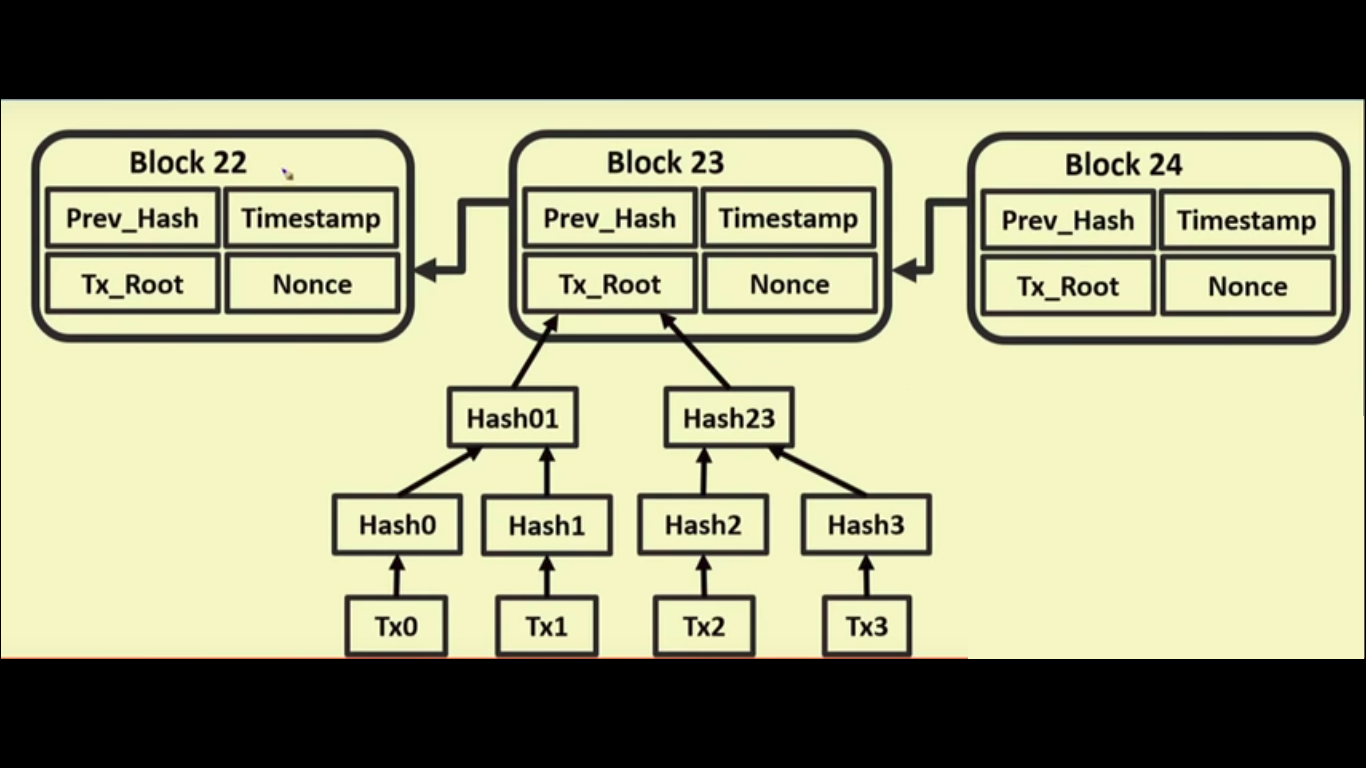
\includegraphics[width=0.75\textwidth]{./img_src/block_chain.png}
\end{center}
\caption{Block Creation}
\end{figure}

\item On request of an image verification, first the image metadata is being checked (1st phase). If the metadata contains the our system generated signature, it will decrypt it and check in that particular block or the range of the blocks for the transaction that contains the image as well as the user's profile for it. Becacuse while creating downloadable file the system encrypts and adds the metadata in the image file. If found, it generates the confirmation message and the links regarding it. And if not then the system requests for time and search the entire blockchain database for hashes (2nd phase). If found it does the same. And still if it not found, it runs a deep CNN for searching for contexts or by object for maximum possible proof (3rd phase). The result it gives now is the final result.
\item The process continues again and again recursively.
\end{enumerate}

\section{Image Comparison Scheme}
The following diagram shows how all the 3 steps the system should follow to chech if an image is already in the system or not \textit{i.e.} Signature Match, Hash Match, Context Match.

The image comparison technique we are trying to build at 3rd level of verification is as follows.
Comparing the two images byte by byte, if the difference between two images is less then the threshold value then image will be same, otherwise we consider that comparison as -(ve) result. To decide the value of threshold we will use machine learning, in which we train our system to decide the threshold value.

\begin{enumerate}
\item We will \q{Get Uploaded Bytes} (GUB) from the file using file uploader api of HTML-5;
\item Then we will try to \q{Extract Metadata} and Search for digital signatures that is expexted to be generated and included by our system;
\item Checking if \q{Signature Found} is true go to 4, else go to 9;
\item Process Signature to get Blocks and Transaction metadata, \textit{i.e.} \textbf{who}, \textbf{where}, \textbf{when} created \textbf{what}.
\item \q{Match Current Metadata with Transactions} (MCMwT) in that Block.
\item If \q{Is Match Found} gives No do nothing, else go for 2nd level matching (next step).
\item \q{Generate Hash} from the image and \q{Match Hash} between the narrowed down two images.
\item If \q{Are Equal} gives true then the Exact match has found, else go for level-3 verification for the two images (discussed in previous paragraph).
\item \q{Generate Hash} for 2nd level verification.
\item \q{Match in All Transactions in All Blocks} for the hash.
\item If \q{Is Found} gives Yes that means an exact match found, else go for level-3 verification for context \q{Match in All Transactions in All Blocks} and it will take a huge amount of time.
\end{enumerate}

\begin{tikzpicture}[node distance=2cm]
\node (start) [startstop] {Start};
\node (in1) [io, right of=start, xshift=2cm] {GUB};
\node (pro1) [process, below of=in1,yshift=0.2cm] {Extract Metadata};
\node (dec1) [decision, below of=pro1, yshift=-0.2cm] {SF};
\node (pro2a) [process, below of=dec1, yshift=-0.2cm] {Process Signature};
\node (pro2b) [process, right of=dec1, xshift=3cm] {Generate Hash};
\node (out1) [process, below of=pro2a] {MCMOT};
\node (check2) [decision,below of=out1,yshift=-0.1cm]{IMF};
\node (ghash) [process, below of=check2,yshift =-0.1cm] {Genrate Hash};
\node (mhash) [process, below of=ghash,yshift = -0.1cm]{Match Hash};
\node (ismhash) [decision, below of=mhash, yshift=-0.1cm]{AE};
%\node (fmatchY) [process, left of=ismhash, xshift = -0.1cm] {YES}
%\node (fmatchN) [process, right of=ismhash, yshift = -0.1cm] {NO}
\node (stop) [startstop, left of=ismhash,xshift= -2cm] {Stop};
\node (m_all_hash) [process, below of=pro2b,yshift=-0.1cm] {MIATIAB};
\node (found2) [decision,below of=m_all_hash,yshift=-0.1cm]{IF};
\node (yes2) [process, below of=found2,yshift =-0.1cm]{Yes};
\node (no2) [process,right of=found2,xshift =2cm]{No};

\draw [arrow] (start) -- (in1);
\draw [arrow] (in1) -- (pro1);
\draw [arrow] (pro1) -- (dec1);
\draw [arrow] (dec1) -- node[anchor=east] {yes} (pro2a);
\draw [arrow] (dec1) -- node[anchor=south] {no} (pro2b);
\draw [arrow] (pro2a) -- (out1);
\draw [arrow] (out1) -- (check2);
\draw [arrow] (check2) -- (ghash);
\draw [arrow] (ghash) -- (mhash);
\draw [arrow] (mhash) -- (ismhash);
\draw [arrow] (ismhash) -- (stop);
\draw [arrow] (pro2b) -- (m_all_hash);
\draw[arrow] (m_all_hash) -- (found2);
\draw [arrow] (found2) -- (yes2);
\draw [arrow] (found2) -- (no2);
\end{tikzpicture}


\chapter{Implementation}
\label{ch:4}
%\setcounter{page}{1}
%\pagenumbering{arabic}
\bigskip

\section{Setup}
\begin{itemize}
\item Computer: Dell, Ubuntu 16.04 LTS
\item Runtime Platform: 1and1 web-server in website \href{https://www.thescienceuniverse.com}{TheScienceUniverse}
\item Server: Localhost, Apache, MySQL, PHP, PHP-MyAdmin
\item Client: Browser (Chrome, FireFox) with HTML-5, CSS-3, JavaScript-5 support, Active Internet Connection
\end{itemize}

\section{Tools}
The list of tools and important functions used:
\begin{itemize}
\item Image API (JS-5 inbuilt)
\item File API (JS-5 inbuilt)
\item SHA-256 (Discussed in \ref{app:1})
\item Base-64 (6 bits encoding scheme replacement of 8 bit executable scheme)
\item Image API with Canvas (JS-5 inbuilt)
\item AES (Discussed in \ref{app:3})
\item RSA (Discussed in \ref{app:2})
\item LR (Discussed in \ref{app:4})
\end{itemize}

We have made basic blockchain platform for a single node processing. The screenshots of the processes are the following steps.
\section{Directory Structure}
The file system we built are as follows, \\
\begin{footnotesize}
blockcain/ -- the root folder \\
|\myTab	index.php -- Home Page (ToDo, News Feed, Others) \\
|\myTab	auth/ -- files for LAMPP authentication system (registration \& login) \\ 
|\myTab	client/ -- files to be run on clients' machine \\
|\myTab |\myTab b\_crt.php -- home page for creating blocks by upload or webcam \\
|\myTab |\myTab b\_upl.php -- upload block directly from client software (NOT BUILT YET) \\
|\myTab |\myTab b\_vrf.php -- verify page by uploading image \\
|\myTab |\myTab profile.php -- profile for user account \\
|\myTab |\myTab mine.php -- mining home for miner account \\
|\myTab |\myTab webcam.php -- use webcam to capture and create transaction to send \\
|\myTab |\myTab upload.php -- use file upload to create and create transaction to send \\
|\myTab |\myTab css/ -- cascading style sheets for home and other pages \\
|\myTab |\myTab js/ -- JavaScript files to be run by browsers \\
|\myTab |\myTab |\myTab script.js -- for index page scripting \\
|\myTab |\myTab |\myTab base.js -- basic function collection \\
|\myTab |\myTab |\myTab sha256.js -- sha256 implementation (Hex String In -- Hex String Out) \\
|\myTab |\myTab |\myTab base64.js -- base64 implementation (codec base 64 String -- base 256 String) \\
|\myTab |\myTab |\myTab upload.js -\} \\
|\myTab |\myTab |\myTab webcam.js -\} get, modify image by canvas, create transaction, send to server \\
|\myTab |\myTab |\myTab verify.js -- scripting for image verification \\
|\myTab |\myTab |\myTab crt\_blk.js -- get data, send to php for creating files \\
|\myTab |\myTab |\myTab mine\_comm.js -- scripting for miners \\
|\myTab	server/ -- server side computation \\
|\myTab |\myTab gfc.php -- get from chain (give data from existing chain) \\
|\myTab |\myTab atc.php -- add to chain (update chain, add file to filesystem) \\
|\myTab |\myTab rtc.php -- real time connect (creating peer-to-peer network with JS-5) \\
|\myTab |\myTab cron.php -- periodic cron task script \\
|\myTab |\myTab vrf.php -- verify chain for security and integrity \\
|\myTab res/ -- the resources  \\
|\myTab |\myTab chain.json -- list of blocks \\
|\myTab |\myTab uvf\_txd/ -- unverified pool of json transactions \\
|\myTab |\myTab tmp\_blk/ -- json blocks held for review \\
|\myTab |\myTab blk/ -- verified and added json blocks \\
\end{footnotesize}

\section{Process Flow}
The process flow in the users' (normal user or miner) perspective is as follows,
\begin{enumerate}
\item User have to be authosized (Figure: \ref{fig:authorize}) means register (sign-up) and log in (sign-in) to the system
\item User becomes a node and gets its home page (Figure: \ref{fig:homepage})
\item There are links to reach Profile (Figure: \ref{fig:profile}), Block Creation (Figure: \ref{fig:img_insert}), Block Uploadation, Image Verification (Figure: \ref{fig:verify}) Pages
\item Profile page consists of users personal details only the user can view and change. If the user is a miner, then the list of blocks created is mentioned in the page and link to mine blocks further.
\item In the home page after clicking on the Block Creation link the user gets on to block creation page (Figure: \ref{fig:img_insert}). Actually the name of the page should be Image Insertion. There are two options (image links for two pages) there, one is WebCam (Figure: \ref{fig:img_webcam}), another is Upload (Figure: \ref{fig:img_upload}) page. \\
WebCam page uses User's webcam after the confirmations from user. It takes real time photo and resizes it in Canvas and gets base64 string for the image pixel values, encrypts it with RSA with server's public key, then creates transaction json structure by following the given rules. \\
Upload page takes image using file uploadation in HTML-5 \& JS-5 file api, gets metadata and stores it, and resizes it in Canvas and gets base64 string for the image pixel and do the same as the webcam script does. \\
Then it sends to server php page using XML-HTTP for further processing. After getting the request server decrypts it using RSA private key, encrypts it with AES and stores it as the transaction json format in unverified pool \textit{i.e.} uvf\_txd/ directory. \\
\item After each 5 minutes the server collects the unverified transactions and publishes to the virtual miners if any of the human miners asked for mining from the mine link included in their profile (Figure: \ref{fig:profile}) page. A human miner gets all the transaction json files downloaded in own computer by PHP and Secure File Transfer Protocol (SFTP). After getting the file it starts verifying the transactions by gossiping with others. After validating the them the miner starts creating the block (Figure: \ref{fig:upload}) until it finishes it or gets another block from the network for verification. As soon as it gets another block for verification it holds own process, and validates it. If it is valid it discards it's own calculation and stores the block in temporary location. If not then it completes creating own block and publish it to the network for the same validation. Up to 5 minutes they gossip in the fully connected graph of peer-to-peer network and reach to a decision which block to keep according to some criteria. After 5 minutes they reach to a final decision and Then it shares the block to server to store as a temporary block.
\item After 5 minutes the server knows that every miner is having mostly choosen copy of the new block after each miner node reaches to a final decision. It validates all and re-check the criteria and gets to a final decision and publishes it to final one to be added in the chain. It then deletes the transactions which are included in the new block from the transaction pool.
\item The server decryps the blocks to get image data and adds in form of canvases in the news feed in Home Page with downloadable link each. After clicking download it creates digital signature and adds in the image metadata for downloading with it, that marks that the image is created in our system.
\item Whenever a peprson goes for image verification (Figure: \ref{fig:verify}) it checks it in 3 steps that is discussed in the image verification portion in Proposal Chapter.
\item The machine learning step comparison \textit{i.e.} step-3, the contextual analysis is interrupted because of some technical limitations that we are going to cover up very soon.
\item Every server file system related works are done in PHP and computational works are done in JS and communicated between them always whenever required.
\end{enumerate}

\section{JSON Files}
\subsection{JSON File Structure}
The JSON (JavaScript Object Notation) files are semi-structured alternate database files inspired by JS object structure. The database structure for the character rules in the file are, \\
File starts and ends with \{ and \} \\
data attributes and values are set in the way, List of key-pair: \\
\q{key} = \q{value}, \ldots
the value can be Number ({0-9}*.{0-9}*), Array ([value, \ldots]), or String (\q{characters}) \\
\noindent \{ \q{officer} = \\
\algoTab \q{name} = \q{ABC XYZ}, \\
\algoTab \q{salary} = 1000.00, \\
\algoTab \q{friends} = [\q{A X}, \q{B Y}, \q{C Z}] \\
\noindent\}

\subsection{JSON Files Used}
The JSON files we are gonna use are,

\subsubsection{txd\_u.json}
-- This file (filename: Unverified Transactions) consists of a list of un-added transactions that are gonna be added in the new block. The JSON file consists of an array named txd, and the attribute fields are the list of following bunch of information for each transaction \\
\textbf{t\_id} Transaction Identifier is created by appending user\_id + \q{\_} + photo\_id, where user\_id is the username, and photo\_id is the Algebra(number of photos the user inserted + 1), \\
\textbf{t\_ts} Transaction Timestamp is the JS generated date-time-location string in an standard format, \\
\textbf{t\_md} Transaction Metadata is the important portion of the metadata in the uploaded digital image file read in hex string of image bytes, \\
\textbf{t\_dh} Transaction Data-Hash is the SHA-256 calculated hex hash string, \\
\textbf{t\_rd} Transaction Raw-Data is the RSA encrypted hex string of Canvas conversion of image bytes.

\subsubsection{blk\_i.json}
-- This file (i in filename: i-th Block is the block number) includes the exact following fields,\\
\textbf{b\_id} Block Identifier is created by appending \q{blk\_} + blk\_id, blk\_id is the Algebra(number of blocks in the chain + 1), \\
\textbf{b\_ts} Block's Timestamp is the JS generated date-time-location string in an standard format, \\
\textbf{b\_ms} Block Miner's Signature, we are currently using creator's user\_name here \\
\textbf{b\_mr} Block's Merkle Root hash is stored in hex string format here \\
\textbf{b\_ph} Block's Previous Hash is the previous block's hash identifier hex string \\
\textbf{b\_ch} Block's Current Hash is the calculated hash of this block, the calculation goes as follows, SHA-256 of (concatinated hex(b\_id, b\_ts, b\_ms), b\_mr, b\_ph), \\
\textbf{b\_dt} Block Data is the list of all the validated transactions' fields that are included in the block; \\

\subsubsection{chain.json} -- This file is the pointer or the book keeper for easy access of the collection of the blocks created. The fields are the list of blocks' information and for each in each entry, \\
\textbf{b\_mn} Block Miner's Signature (discussed earlier) \\
\textbf{b\_fn} Block's File-Name is created by appending \q{blk\_} + i from b\_id + \q{.json} which is stored in the same resource directory \\
\textbf{c\_ch} Chain's Current Hash is the last block's current hash (b\_ch) to keep an eye on the last block \\

\begin{figure}
\begin{center}
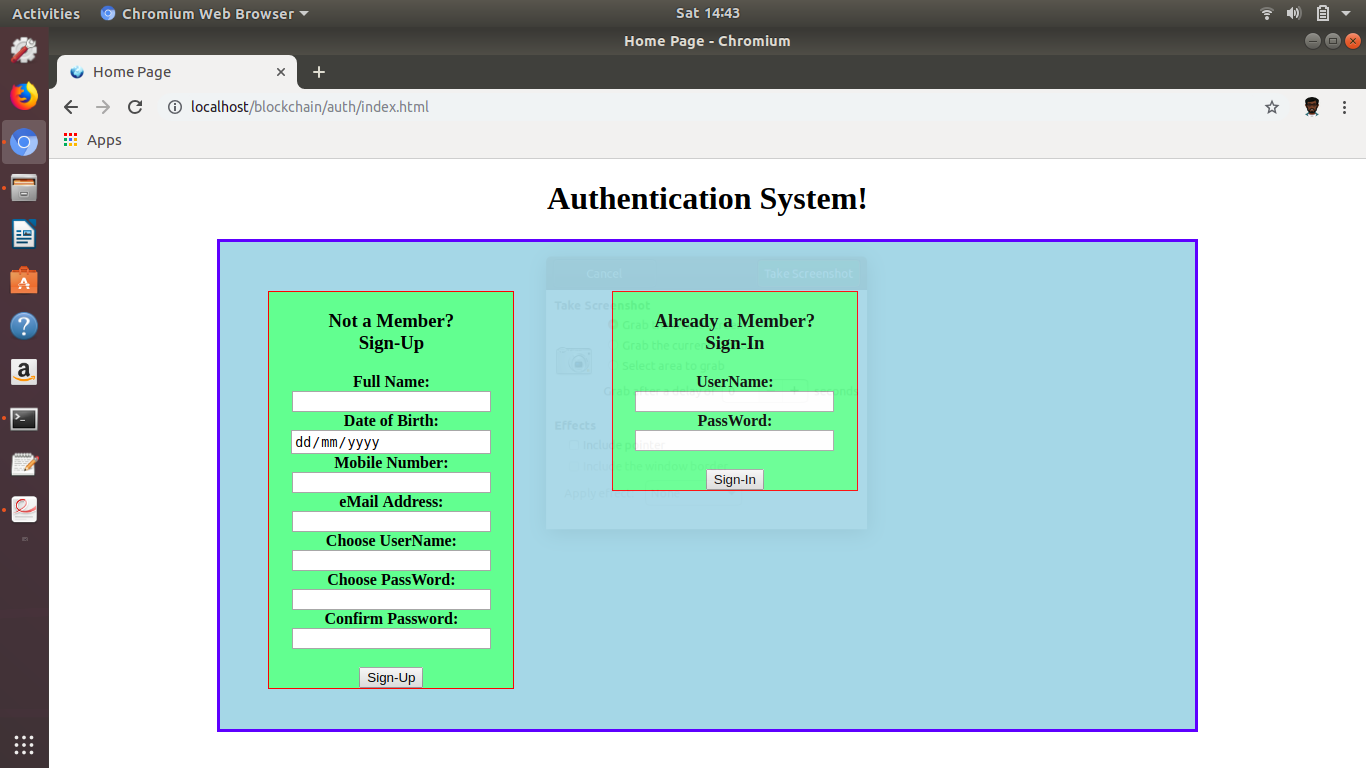
\includegraphics[width=0.75\textwidth]{./img_src/screen0.png}
\end{center}
\caption{Authentication Page}
\label{fig:authorize}
\end{figure}

\begin{figure}
\begin{center}
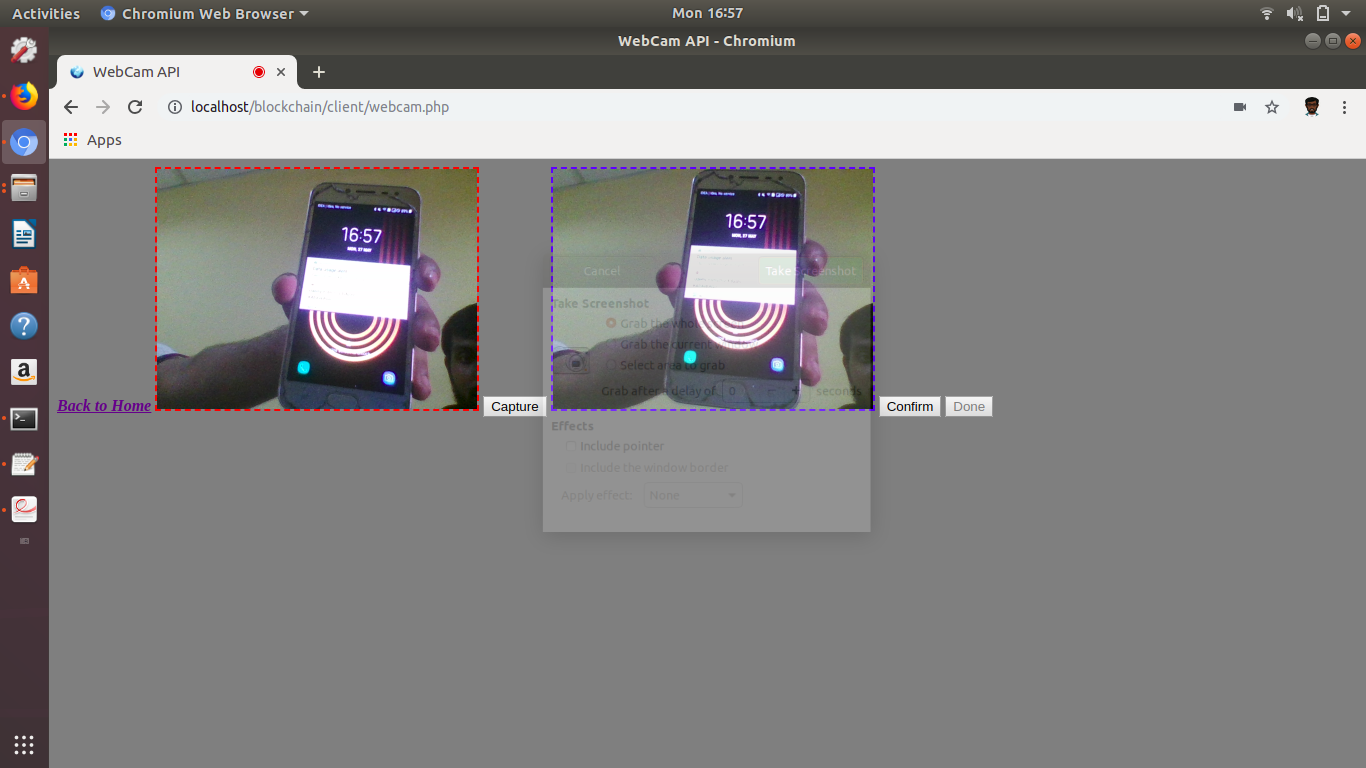
\includegraphics[width=0.75\textwidth]{./img_src/screen1.png}
\end{center}
\caption{Home Page}
\label{fig:homepage}
\end{figure}

\begin{figure}
\begin{center}
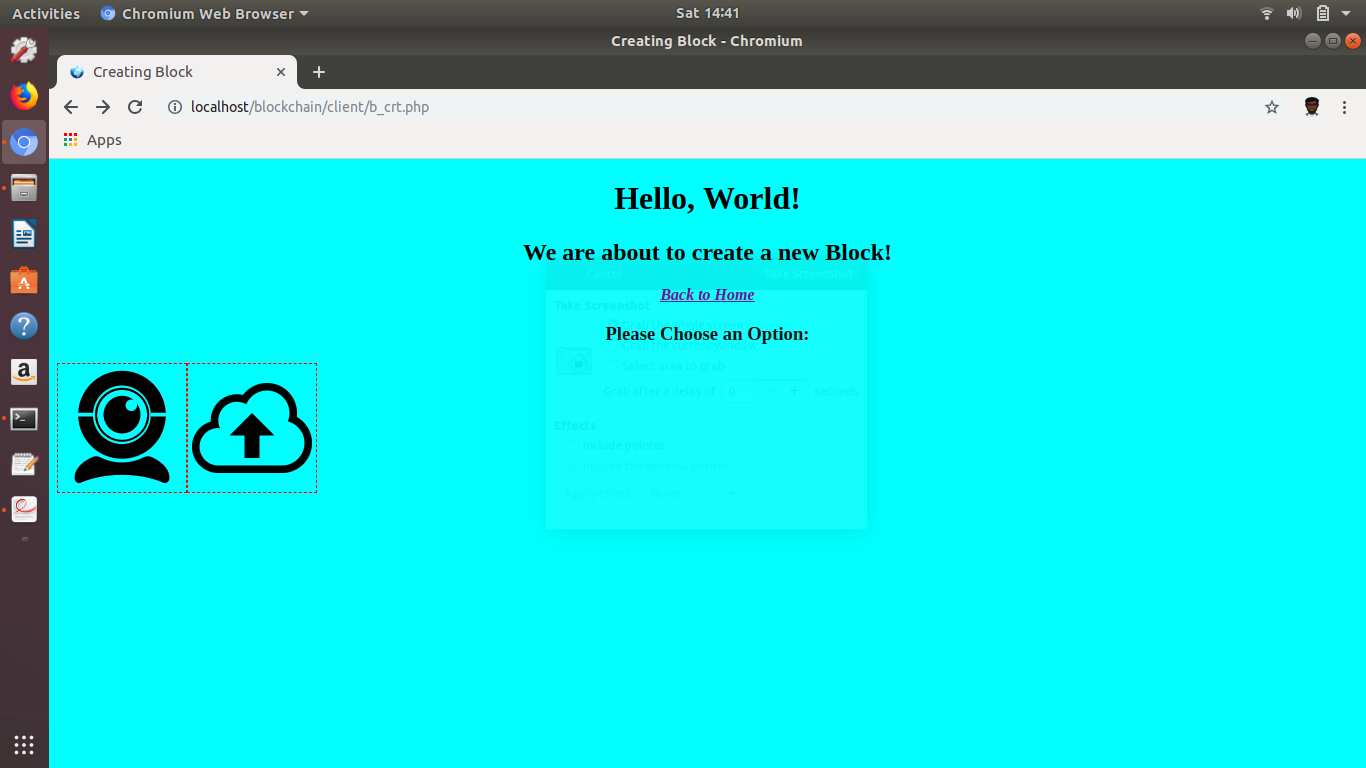
\includegraphics[width=0.75\textwidth]{./img_src/screen2.png}
\end{center}
\caption{Choose How to Insert Image}
\label{fig:img_insert}
\end{figure}

\begin{figure}
\begin{center}
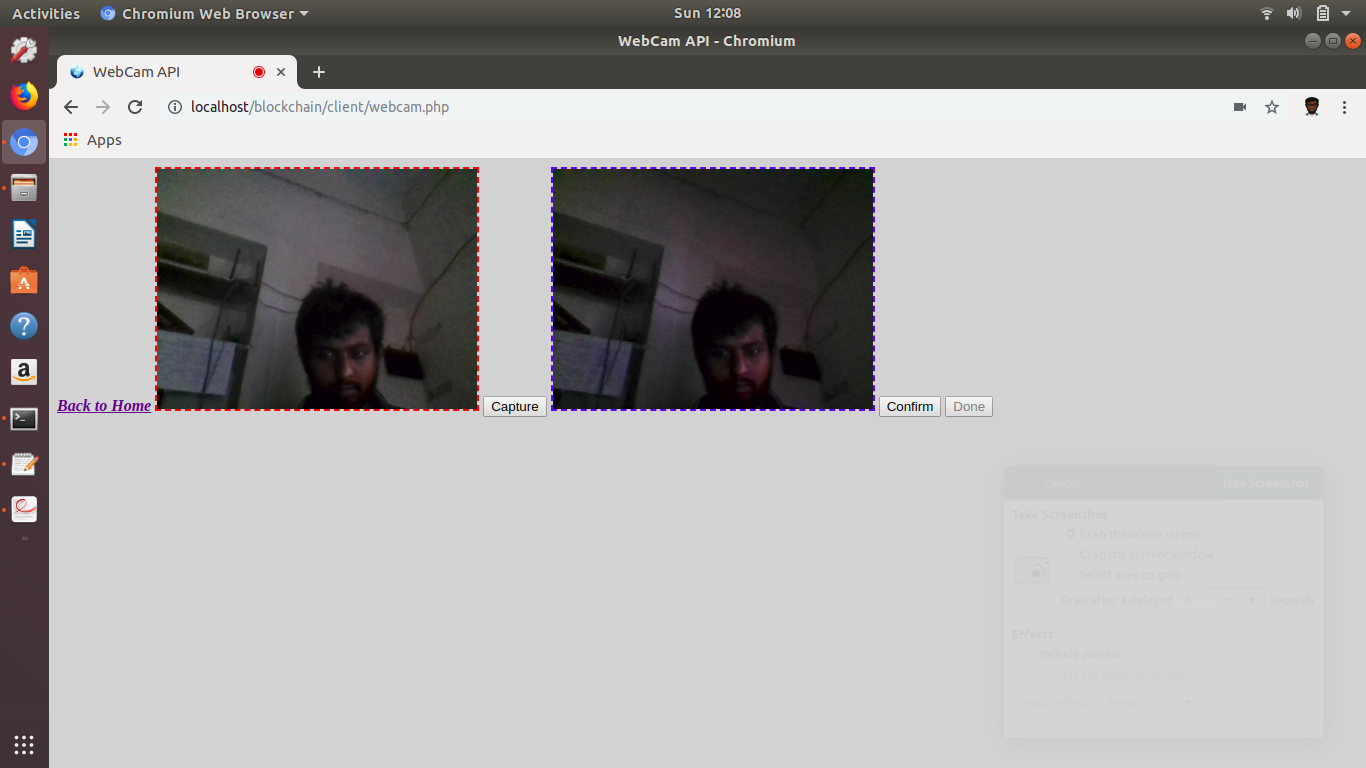
\includegraphics[width=0.75\textwidth]{./img_src/screen3.png}
\end{center}
\caption{WebCam}
\label{fig:img_webcam}
\end{figure}

\begin{figure}
\begin{center}
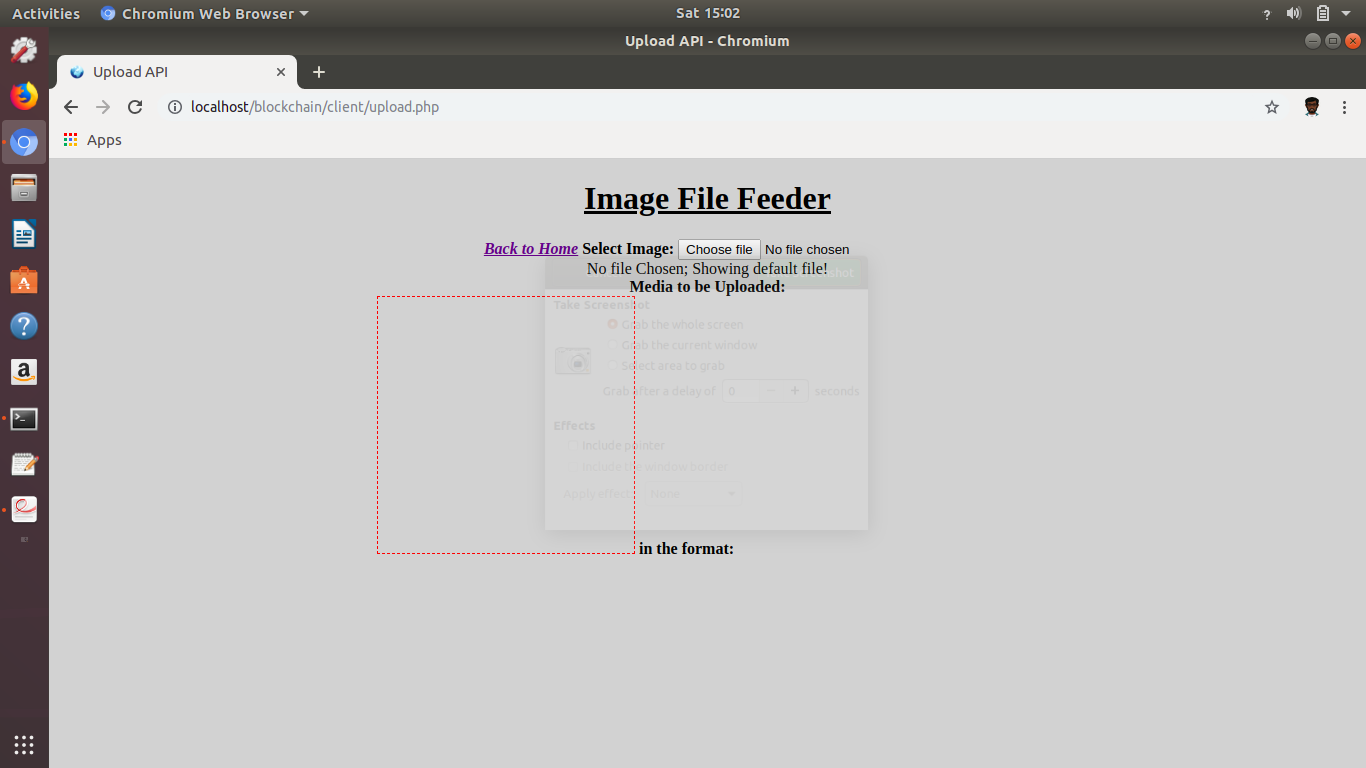
\includegraphics[width=0.75\textwidth]{./img_src/screen4.png}
\end{center}
\caption{Upload}
\label{fig:img_upload}
\end{figure}

\begin{figure}
\begin{center}
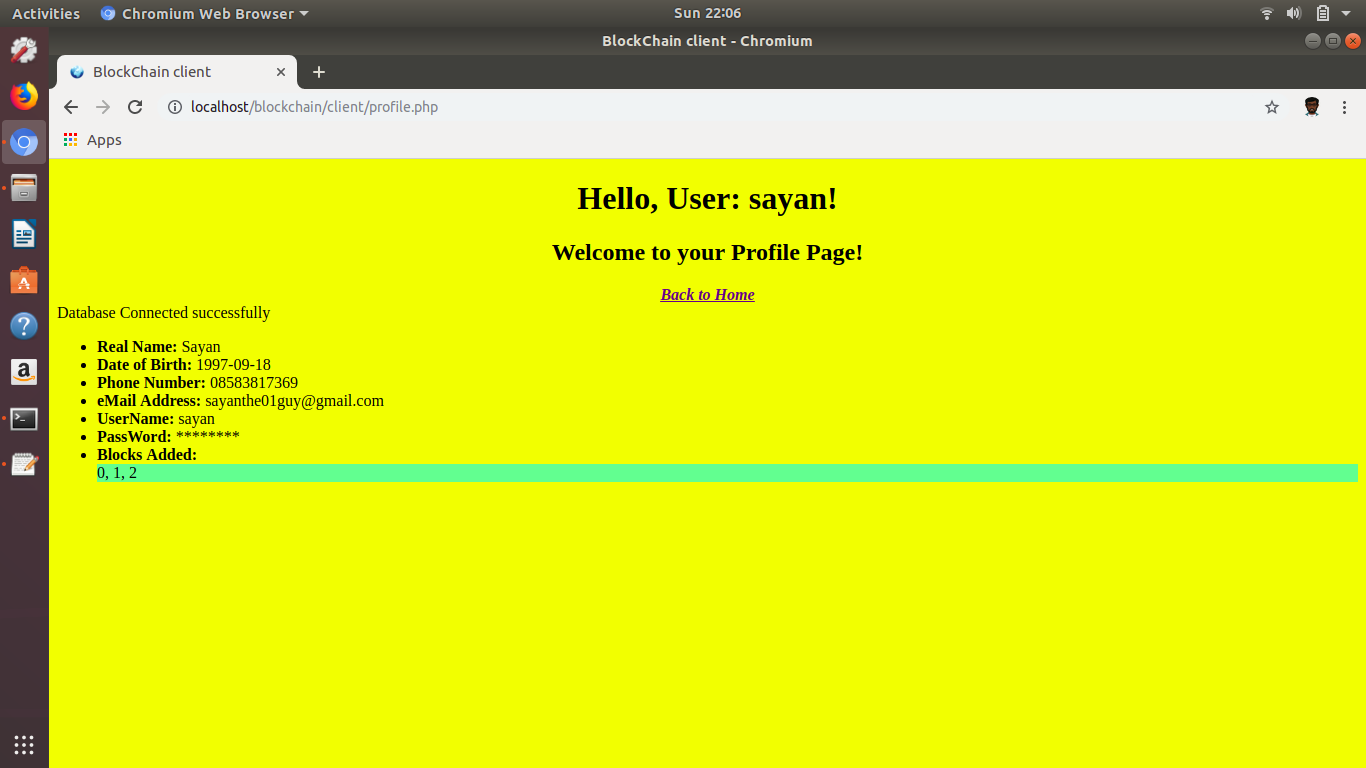
\includegraphics[width=0.75\textwidth]{./img_src/screen5.png}
\end{center}
\caption{Profile}
\label{fig:profile}
\end{figure}

\begin{figure}
\begin{center}

\includegraphics[width=0.75\textwidth]{./img_src/upload.png}
\end{center}
\caption{Image Insertion}
\label{fig:upload}
\end{figure}

\begin{figure}
\begin{center}
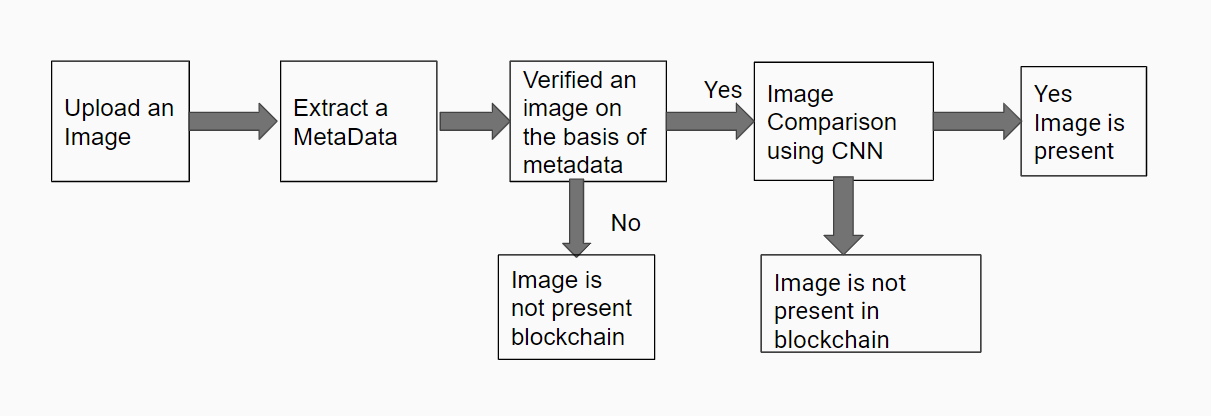
\includegraphics[width=0.75\textwidth]{./img_src/verify.png}
\end{center}
\caption{Image Verification}
\label{fig:verify}
\end{figure}

\chapter{Conclusion and Further Work}
\label{Ch6} This synopsis provides a detailed description of an Practical implementation of Online Biding system which provides Secure Key Exchange and agreement. We have implemented system for
\begin{itemize}
\item Capturing or uploading image;
\item Show status in Home and Profile Page;
\item Processing the image;
\item Signing the image
\item Create transactions
\item Create block in server
\item Adding to chain
\end{itemize}

\subsubsection{Further Work}
The next targets are to create a system that will standalone perform the following tasks
\begin{itemize}
\item making a peer-to-peer network for android that will perform the following tasks
\item connecting to Online Verifier service
\item sending and Receive messages containing data between peers
\item improving Verification Service
\item connecting in mobile application
\item estimating risks and reconfigure concensus protocols
\end{itemize}

\cite{nakamoto2008bitcoin, adam_fabian}
\cite{blockchain_wiki}
\bibliographystyle{plain}
\bibliography{./doc_src/reference.bib}


\end{document}
